\documentclass[10pt,a4paper]{article}
\usepackage[utf8]{inputenc}

\title{Package \textsf{dsdraw}}
\author{Jander Moreira}

\usepackage[sourcecodepro]{dsdraw}

\usepackage{tikz}
\usetikzlibrary{decorations.pathreplacing}

\usepackage{tcolorbox}
\tcbuselibrary{listingsutf8, skins, breakable}
\usepackage{listings}
\tcbset{
    colback = black!10,
    colframe = black!30,
    bicolor,
    breakable,
    colbacklower = white,
    listing options = {
        language = {[LaTeX]TeX},
        basicstyle = \ttfamily\scriptsize,
        aboveskip = 0pt,
        belowskip = 0pt,
        tabsize = 2,
    }
}

\RequirePackage{listings}
\lstset{
    literate=
        {á}{{\'a}}1 {é}{{\'e}}1 {í}{{\'i}}1 {ó}{{\'o}}1 {ú}{{\'u}}1
        {Á}{{\'A}}1 {É}{{\'E}}1 {Í}{{\'I}}1 {Ó}{{\'O}}1 {Ú}{{\'U}}1
        {à}{{\`a}}1 {è}{{\`e}}1 {ì}{{\`i}}1 {ò}{{\`o}}1 {ù}{{\`u}}1
        {À}{{\`A}}1 {È}{{\'E}}1 {Ì}{{\`I}}1 {Ò}{{\`O}}1 {Ù}{{\`U}}1
        {ä}{{\"a}}1 {ë}{{\"e}}1 {ï}{{\"i}}1 {ö}{{\"o}}1 {ü}{{\"u}}1
        {ã}{{\~a}}1 {õ}{{\~o}}1
        {Ã}{{\~A}}1 {Õ}{{\~O}}1
        {Ä}{{\"A}}1 {Ë}{{\"E}}1 {Ï}{{\"I}}1 {Ö}{{\"O}}1 {Ü}{{\"U}}1
        {â}{{\^a}}1 {ê}{{\^e}}1 {î}{{\^i}}1 {ô}{{\^o}}1 {û}{{\^u}}1
        {Â}{{\^A}}1 {Ê}{{\^E}}1 {Î}{{\^I}}1 {Ô}{{\^O}}1 {Û}{{\^U}}1
        {ç}{{\c c}}1 {Ç}{{\c C}}1
        {ø}{{\o}}1 {å}{{\r a}}1 {Å}{{\r A}}1
        {œ}{{\oe}}1 {Œ}{{\OE}}1 {æ}{{\ae}}1 {Æ}{{\AE}}1
    %{ß}{{\ss}}1
        {ű}{{\H{u}}}1 {Ű}{{\H{U}}}1 {ő}{{\H{o}}}1 {Ő}{{\H{O}}}1
        {£}{{\pounds}}1
    %{«}{{\guillemotleft}}1
    %{»}{{\guillemotright}}1
        {ñ}{{\~n}}1 {Ñ}{{\~N}}1 {¿}{{?`}}1
}

\newcommand*{\specname}[1]{\mbox{$\langle$\textsl{#1}$\rangle$}}
\newcommand{\library}[1]{%
    \tikz[anchor = base, baseline, outer sep = 0pt, inner sep = 0pt]\node[font = \ttfamily,
        inner ysep = 0.1em, inner xsep = 0.2em,
        transform shape, scale = 0.8,
        text height = 1em,
        text depth = 0.25ex,
        fill = orange!30, %draw, thick,
        rounded corners = 0.2em] {#1};%
}

\begin{document}
\sloppy
\maketitle

%
%\section{Commands}
%
%Easy of use:
%
%\section{Symbols}
%
%\foreach \sym in {NullSymb, EmptySymb}{
%	\noindent \texttt{\textbackslash\sym}: \csname\sym\endcsname\par
%}
%


\section{Libraries}


\subsection{\protect\library{record}}
Drawing records and fields.
\usedslibrary{record}

\subsubsection{Records and fields}
Record structure with field names and byte offsets:
\begin{tcblisting}{}
\usedslibrary{record}
\begin{tikzpicture}
	\dsrecordstructure{%
		name/15,       % 15 bytes
		status/1,      % single byte, label won't fit
		n/2,           % two bytes, label fits,
		phone/30/10,   % 30 bytes, but draws with 10
		e-mail/50/20   % 30 bytes, but draws with 20
	}
\end{tikzpicture}\par
\vspace{1em}
\begin{tikzpicture}
	\dsrecordstructure{%
		name/15,       % 15 bytes
		status/1/6,    % single byte, but draws with 6; label fits now
		n/2,           % two bytes, label fits,
		phone/30/10,   % 30 bytes, but draws with 10
		e-mail/50/20   % 30 bytes, but draws with 20
	}
\end{tikzpicture}
\end{tcblisting}

Field with contents:
\begin{tcblisting}{}
\begin{tikzpicture}[]
	% fields must be placed inside dsrecord environments
	\begin{dsrecord}
		\dsfield{John~Taylor} % spaces must be explicit
	\end{dsrecord}

	% starred version hides outer border
	\begin{dsrecord*}[][yshift = -2.5em] 
		\dsfield{John~Taylor} 
	\end{dsrecord*}

	\begin{dsrecord*}[][yshift = -5em] 
		\dsfield*{John~Taylor} % \dsfield* is a compact version (looks ugly)
	\end{dsrecord*}
\end{tikzpicture}
\end{tcblisting}

When field contents use UTF-8 encoded characters, such as ``á'' and ``ñ'', they are represented by their two-byte encoding in hexadecimal.

\begin{tcblisting}{}
\begin{tikzpicture}[]
	\begin{dsrecord}
		\dsfield{João~Afrânio}
	\end{dsrecord}
\end{tikzpicture}

\begin{tikzpicture}[]
	\begin{dsrecord}
		\dsfield{Jo{ã}o~Afr{â}nio}
	\end{dsrecord}
\end{tikzpicture}
\end{tcblisting}


Field with contents using a terminator (default: \texttt{0x00}):
\begin{tcblisting}{}
\begin{tikzpicture}[]
	\begin{dsrecord*}
		\dsfieldterminator{John~Taylor}
	\end{dsrecord*}

	\begin{dsrecord*}[][yshift = -2.5em]
		\dsfieldterminator{John~Taylor}[*] % new terminator
	\end{dsrecord*}
\end{tikzpicture}
\end{tcblisting}

Field with contents using binary length prefix (big endian with 2 bytes):
\begin{tcblisting}{}
\begin{tikzpicture}[]
	\begin{dsrecord*}
		\dsfieldprefixed{John~Taylor}
	\end{dsrecord*}
\end{tikzpicture}
\end{tcblisting}

Field with contents using fixed size (unused bytes are all set to \texttt{0xFF}):
\begin{tcblisting}{}
\begin{tikzpicture}[]
	\begin{dsrecord*}
		\dsfieldfixed{15}{John~Taylor}
	\end{dsrecord*}
\end{tikzpicture}
\end{tcblisting}

Starred field commands typeset in a compact form:
\begin{tcblisting}{}
\begin{tikzpicture}[]
	\begin{dsrecord*}
		\dsfieldprefixed{John~Taylor}
	\end{dsrecord*}
	
	\begin{dsrecord*}[][yshift = -2.5em)]
		\dsfieldprefixed*{John~Taylor}
	\end{dsrecord*}
\end{tikzpicture}
\end{tcblisting}

Records are groups of fields:
\begin{tcblisting}{}
\begin{tikzpicture}[]
	\begin{dsrecord}
		\dsfieldprefixed*{John~Taylor}   % name
		\dsfieldfixed*{2}{NY}            % state
		\dsfieldfixed*{10}{08/23/1988}   % birth date
	\end{dsrecord}

	\begin{dsrecord}[][yshift = -1cm]
		\dsfieldprefixed*{John~Taylor}
		\dsfieldspace
		\dsfieldfixed*{2}{NY}
		\dsfieldspace
		\dsfieldfixed*{10}{08/23/1988}
	\end{dsrecord}

	\begin{dsrecord*}[][yshift = -2cm]
		\dsfieldprefixed*{John~Taylor}
		\dsfieldspace
		\dsfieldfixed*{2}{NY}
		\dsfieldspace
		\dsfieldfixed*{10}{08/23/1988}
	\end{dsrecord*}
\end{tikzpicture}
\end{tcblisting}

Records with terminator (default: \texttt{0x01}):
\begin{tcblisting}{}
\begin{tikzpicture}[]
	\begin{dsrecord}[terminator]
		\dsfieldprefixed*{John~Taylor}
		\dsfieldfixed*{2}{NY}
		\dsfieldfixed*{10}{08/23/1988}
	\end{dsrecord}
\end{tikzpicture}
\end{tcblisting}

Records with binary length prefix (little endian with 2 bytes):
\begin{tcblisting}{}
\begin{tikzpicture}[]
	\begin{dsrecord}[prefix]
		\dsfieldprefixed*{John~Taylor}
		\dsfieldfixed*{2}{NY}
		\dsfieldfixed*{10}{08/23/1988}
	\end{dsrecord}
\end{tikzpicture}
\end{tcblisting}


Records with fixed length (unused bytes are set to \texttt{0xFE}):
\begin{tcblisting}{}
\begin{tikzpicture}[]
	\begin{dsrecord}[length = 40]
		\dsfieldprefixed*{John~Taylor}
		\dsfieldfixed*{2}{NY}
		\dsfieldfixed*{10}{08/23/1988}
	\end{dsrecord}
	
	\begin{dsrecord}[length = 50][yshift = -1cm]
		\dsfieldprefixed*{John~Taylor}
		\dsfieldfixed*{2}{NY}
		\dsfieldfixed*{10}{08/23/1988}
	\end{dsrecord}
\end{tikzpicture}
\end{tcblisting}

When a record is marked as deleted, its first eight bytes as set to:
\begin{itemize}
	\item Two bytes to tell the total length of available space (big endian);
	\item The two-byte magic number \texttt{0xFFFF} that states ``deleted'';
	\item An optional four-byte address used in linked lists as a ``next'' field (big endian).
\end{itemize}
\begin{tcblisting}{}
\begin{tikzpicture}
	\begin{dsrecord}[terminator]
		\dsfieldterminator*{John~Taylor}
		\dsfieldspace
		\dsfieldprefixed*{2}{NY}
		\dsfieldspace
		\dsfieldfixed*{10}{08/23/1988}
	\end{dsrecord}
	\begin{dsrecord}[terminator, deleted][yshift = -2.5em]
		\dsfieldterminator*{John~Taylor}
		\dsfieldspace
		\dsfieldprefixed*{2}{NY}
		\dsfieldspace
		\dsfieldfixed*{10}{08/23/1988}
	\end{dsrecord}
	\begin{dsrecord}[terminator, deleted, next = 0xDA4][yshift = -5em]
		\dsfieldterminator*{John~Taylor}
		\dsfieldspace
		\dsfieldprefixed*{2}{NY}
		\dsfieldspace
		\dsfieldfixed*{10}{08/23/1988}
	\end{dsrecord}
\end{tikzpicture}
\end{tcblisting}


To save effort, a new record structure can be defined.
\begin{tcblisting}{}
\dsnewnamedrecord{record_one}{
	\dsfieldprefixed*,
	\dsfieldspace\dsfieldfixed*{2},
	\dsfieldspace\dsfieldfixed*{10}
}

\dsnewnamedrecord{record_two}{
	\dsfieldfixed*{20},
	\dsfieldspace\dsfieldfixed*{2},
	\dsfieldspace\dsfieldfixed*{10}
}


\begin{tikzpicture}
	\dsnamedrecord{record_one}{John~Taylor, NY, 08/23/1988}
\end{tikzpicture}

\begin{tikzpicture}
	\dsnamedrecord[prefix]{record_one}{Michael~Smith, TX, 01/18/2001}
\end{tikzpicture}

\begin{tikzpicture}
	\dsnamedrecord[terminator]{record_two}{José~João~Afrânio, SP, 11/03/1944}
\end{tikzpicture}

\begin{tikzpicture}
	\dsnamedrecord[deleted, terminator]{record_two}{José~João~Afrânio, SP,
		11/03/1944}
\end{tikzpicture}
\end{tcblisting}

\subsubsection{References}

A record structure can be named (default name is \textit{record}) and each field is named \specname{record name}\texttt{-field-}$n$, starting at zero. Whenever possible, also the field names can be used.

\begin{tcblisting}{}
\usedslibrary{record}
\begin{tikzpicture}[remember picture]
	\dsrecordstructure[name = {my record}, % name a record
		hide structure offsets]{name/15, status/1, n/2, phone/30/15,
			e-mail/50/20}
	
	\foreach \f[count = \n] in {field-0, field-3, e-mail, phone}{
		\draw[latex-, font = \scriptsize]
			(my record-\f) -- ++(-1em, -\n * 1.2em - 1em)
			node[below] {\texttt{(my record-\f)}};
	}
	
	\draw[latex-, font = \scriptsize] (my record) -- ++(1em, 2em)
		node[above] {\texttt{(my record)}};
\end{tikzpicture}\par
\end{tcblisting}

Records with contents are also named and have the following labels alongside the whole record:
\begin{itemize}
	\item Each byte is \specname{record name}\texttt{-byte-}$n$ ($n \geq 0$);
	\item Each field is \specname{record name}\texttt{-field-}$n$ ($n \geq 0$);
\end{itemize}

\begin{tcblisting}{}
\begin{tikzpicture}
	\begin{dsrecord}
		\dsfieldterminator*{John~Taylor}
		\dsfieldspace
		\dsfieldprefixed*{2}{NY}
		\dsfieldspace
		\dsfieldfixed*{10}{08/23/1988}
	\end{dsrecord}
	
	\draw[latex-, thick] (record) -- ++(2em, -6em)
		node[font = \scriptsize, below] {\texttt{(record)}};

	\foreach \f in {0, 1, 2}{
		\draw[latex-]
			(record-field-\f) -- ++(\f * 1em - 2em, \f * 1.2em + 2em)
			node[font = \scriptsize, above] {\texttt{(record-field-\f)}};
	}
	
	\foreach \b[count = \n] in {0, 1, 2, 4, 11, 12, 22, 23, 24}{
		\draw[latex-]
			(record-byte-\b.south) -- ++(-0.5em, \n * -1.2em - 1em)
			-- ++(-1em, 0)
			node[font = \scriptsize, below left,
				anchor = east] {\texttt{(record-byte-\b)}};
	}
\end{tikzpicture}
\end{tcblisting}

Some record organization bytes are also labelled (if present):
\begin{itemize}
	\item the record terminator (\specname{record name}\texttt{-terminator});
	\item the prefixed record size (\specname{record name}\texttt{-prefix});
	\item the fragmentation of fixed length records (\specname{record name}\texttt{-fragmentation}).
\end{itemize}

\begin{tcblisting}{}
\begin{tikzpicture}[]
	\begin{dsrecord}[terminator]
		\dsfieldterminator*{John~Taylor}
		\dsfieldspace
		\dsfieldprefixed*{2}{NY}
		\dsfieldspace
		\dsfieldfixed*{10}{08/23/1988}
	\end{dsrecord}
	\draw[latex-, font = \scriptsize] (record-terminator) -- ++ (1em, 2em)
		node[above]{\texttt{(record-terminator)}};

	\begin{dsrecord}[prefix][yshift = -2.5em]
		\dsfieldterminator*{John~Taylor}
		\dsfieldspace
		\dsfieldprefixed*{2}{NY}
		\dsfieldspace
		\dsfieldfixed*{10}{08/23/1988}
	\end{dsrecord}
	\draw[latex-, font = \scriptsize] (record-prefix) -- ++ (-2em, 1em)
		node[left]{\texttt{(record-prefix)}};

	\begin{dsrecord}[length = 30][yshift = -5em]
		\dsfieldterminator*{John~Taylor}
		\dsfieldspace
		\dsfieldprefixed*{2}{NY}
		\dsfieldspace
		\dsfieldfixed*{10}{08/23/1988}
	\end{dsrecord}
	\draw[decorate,
		decoration = {brace, mirror, amplitude = 0.4em, raise = 0.3em}]
		(record-fragmentation.south west) --
		(record-fragmentation.south east)
		node[font = \scriptsize,
			midway, yshift = -1.5em]{\texttt{(record-fragmentation)}};
\end{tikzpicture}
\end{tcblisting}

a
%

\subsection{Library \protect\library{file}}
The library \library{file} draws files and uses \library{record}.

\usedslibrary{file}

\subsubsection{Drawing files horizontally}
Horizontal file with records.




\begin{tcblisting}{}
\begin{tikzpicture}
	\dsfilestructure[block size = 4096, kbyte width = 15em,
		structure offsets
	]{
		R$_0$/500,
		R$_1$/1300,
		R$_2$/1800,
		R$_3$/900,
		R$_4$/850
	}
\end{tikzpicture}
\end{tcblisting}


\subsubsection{Drawing files vertically}

Files and records are drawn in vertical mode, one record at a time. All records must be defined with \verb|\dsnewnamedrecord| and multiple record formats can be used. \verb|\dsfilenamedrecord| is used to put each record.

\begin{tcblisting}{}
\dsnewnamedrecord{fixed_length}{
	\dsfieldfixed*{12},
	\dsfieldfixed*{2},
	\dsfieldfixed*{18}
}
\dsnewnamedrecord{variable_length}{
	\dsfieldterminator*,
	\dsfieldprefixed*
}

\begin{tikzpicture}[]
	\usedslibrary{file}

	% environment for a file
	\begin{dsfile}
		\dsfilenamedrecord{fixed_length}{Grace, 22, UK}
		\dsfilenamedrecord{fixed_length}{Roberta, 31, Brazil},
		\dsfilenamedrecord{variable_length}{Karl~Ulrich, Germany},
		\dsfilenamedrecord{fixed_length}{Bethany, 34, USA}
		\dsfilenamedrecord{variable_length}{Sandoval, Chile},
	\end{dsfile}
\end{tikzpicture}
\end{tcblisting}


If all records share the same format, \verb|\dsfilerecords| can be used to set records in an easier way. Both \verb|\dsfilerecords| and \verb|\dsfilenamedrecord| can be intermixed.

\begin{tcblisting}{}
\dsnewnamedrecord{record}{
	\dsfieldfixed*{12},
	\dsfieldspace\dsfieldfixed*{2},
	\dsfieldspace\dsfieldfixed*{18}
}

\begin{tikzpicture}[]
	\begin{dsfile}[show frame, show offsets]
		\dsfilerecords{record}{
			{Grace, 22, UK},
			{Roberta, 31, Brazil},
			{Ulrich, 12, Germany},
			{Bethany, 34, USA}
		}
	\end{dsfile}
\end{tikzpicture}
\end{tcblisting}

Blocks

\begin{tcblisting}{}
\dsnewnamedrecord{record}{
	\dsfieldfixed*{12},
	\dsfieldspace\dsfieldfixed*{2},
	\dsfieldspace\dsfieldfixed*{18}
}

\begin{tikzpicture}
	\begin{dsfile}[records = 5, show offsets]
		\begin{dsblock}{record}
			\dsfilerecords{record}{
				{Grace, 22, UK},
				{Roberta, 31, Brazil}
			}
		\end{dsblock}

		\begin{dsblock}{record}
			\dsfilerecords{record}{
				{Karl, 18, Germany},
				{Ulrich, 12, Germany},
				{Bethany, 34, USA}
			}
		\end{dsblock}
	\end{dsfile}
\end{tikzpicture}
\end{tcblisting}


\subsubsection{References}

\begin{tcblisting}{}
\dsnewnamedrecord{record}{
	\dsfieldfixed*{15},
	\dsfieldfixed*{2},
	\dsfieldfixed*{14}
}

\begin{tikzpicture}[]
	\begin{dsfile}[hide offsets]
		\dsfilerecords{record}{
			{Grace, 22, UK},
			{Roberta~Souza, 31, Brazil/name = important},
			{Ulrich, 12, Germany},
			{Bethany, 34, USA}
		}
	\end{dsfile}

	\draw[latex-] (important.east) -- ++(3em, 3em)
		node[above, font = \scriptsize] {\texttt{(important.east)}};
	\foreach \n in {0, ..., 3}{
		\draw[latex-] (file-record-\n) -- ++(-9.5em, -\n * 1.2em + 1.5em)
			node[left, font = \scriptsize] {\texttt{(file-record-\n)}};
	}
	\draw[latex-, thick] (important-field-1) -- ++(1em, 4em)
		node[above, font = \scriptsize] {\texttt{(important-field-1)}};
	\draw[latex-, thick] (file-record-3-field-2) -- ++(-1.5em, -2em)
		node[below, font = \scriptsize] {\texttt{(file-record-3-field-2)}};
\end{tikzpicture}
\end{tcblisting}




    %\ExplSyntaxOn
    %\str_set_convert:Nnnn \l_latin_str {ação} {utf8} {latin1}
    %\str_map_inline:Nn \l_latin_str {(##1)}
    %
    %\ExplSyntaxOff


\end{document}